%%%%%%%%%%%%%%%%%%%%%%%%%%%%%%%%%%%%%%%%%
% a0poster Portrait Poster 
% LaTeX Template
% with University Copenhagen logo
% Version 1.0 (22/06/13)
%
% Based on:
% The a0poster class was created by:
% Gerlinde Kettl and Matthias Weiser (tex@kettl.de)
% 
% This template has been downloaded from:
% http://www.LaTeXTemplates.com
%
%%%%%%%%%%%%%%%%%%%%%%%%%%%%%%%%%%%%%%%%%

%----------------------------------------------------------------------------------------
%	PACKAGES AND OTHER DOCUMENT CONFIGURATIONS
%----------------------------------------------------------------------------------------

\documentclass[a0,portrait]{a0poster}
\usepackage[utf8]{inputenc}

\usepackage{multicol} % This is so we can have multiple columns of text side-by-side
\columnsep=100pt % This is the amount of white space between the columns in the poster
\columnseprule=3pt % This is the thickness of the black line between the columns in the poster

\usepackage[svgnames]{xcolor} % Specify colors by their 'svgnames', for a full list of all colors available see here: http://www.latextemplates.com/svgnames-colors

\usepackage{times} % Use the times font
%\usepackage{palatino} % Uncomment to use the Palatino font

\usepackage{graphicx} % Required for including images
\graphicspath{{figures/}} % Location of the graphics files
\usepackage{booktabs} % Top and bottom rules for table
\usepackage[font=small,labelfont=bf]{caption} % Required for specifying captions to tables and figures
\usepackage{amsfonts, amsmath, amsthm, amssymb} % For math fonts, symbols and environments
\usepackage{wrapfig} % Allows wrapping text around tables and figures
\definecolor{ku}{RGB}{144,26,30}
\definecolor{ku-yellow}{RGB}{255,249,25}
\usepackage{subfig}


\begin{document}
%----------------------------------------------------------------------------------------
%	POSTER HEADER 
%----------------------------------------------------------------------------------------

% The header is divided into two boxes:
% The first is 75% wide and houses the title, subtitle, names, university/organization and contact information
% The second is 25% wide and houses a logo for your university/organization or a photo of you
% The widths of these boxes can be easily edited to accommodate your content as you see fit



\begin{minipage}[t]{0.60\linewidth}
\vspace{0.1cm}
\begin{flushleft}
	\Huge \color{ku} \textbf{Planning genetic algorithms to compose	music} \color{Black}\\ % Title
\LARGE\textbf{Aytug Altin} - \Large Bachelor of computer science % 
\end{flushleft}


\end{minipage}
%
\begin{minipage}[t]{0.40\linewidth}
\vspace{0.1cm}
\flushright
\begin{center}
	
\includegraphics[width=0.6\linewidth]{UHasselt-liggend}
\end{center}
\end{minipage}


%----------------------------------------------------------------------------------------

\begin{multicols}{2} % This is how many columns your poster will be broken into, a portrait poster is generally split into 2 columns

%----------------------------------------------------------------------------------------
%	ABSTRACT
%----------------------------------------------------------------------------------------



%----------------------------------------------------------------------------------------
%	INTRODUCTION
%----------------------------------------------------------------------------------------

\color{SaddleBrown} % SaddleBrown color for the introduction
\begin{flushleft}
\Large{\textbf{Introduction}}
\end{flushleft}
\large{We \textbf{simulated} a nature where \textbf{songs try to survive} with one another by using the principle behind the \textbf{genetic algorithm}. The genetic algorithm takes a number of \textbf{parents}, \textbf{crosses} them with each other and \textbf{selects} the \textbf{best results}. Crossing two songs will result in a combination of both of them in a random structure. Rating them is based on a \textbf{predefined theory} or a set of rules. Mutations are both \textbf{planned and random}.}

%----------------------------------------------------------------------------------------
%	OBJECTIVES
%----------------------------------------------------------------------------------------

\color{DarkSlateGray} % DarkSlateGray color for the rest of the content



\begin{flushleft}
	\Large{\textbf{Application Structure}}
\end{flushleft}
\vspace{0.1cm}
\begin{center}
	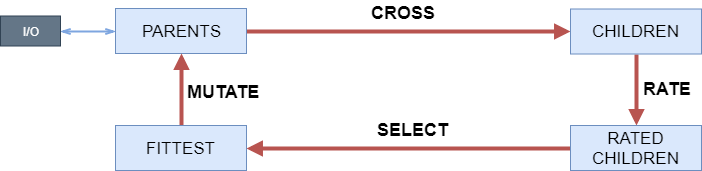
\includegraphics[width=\linewidth]{App_structure}
\end{center}

%----------------------------------------------------------------------------------------
%	MATERIALS AND METHODS
%----------------------------------------------------------------------------------------

\begin{flushleft}
	\Large{\textbf{Crossover}}
\end{flushleft}
\vspace{0.1cm}
\begin{center}
	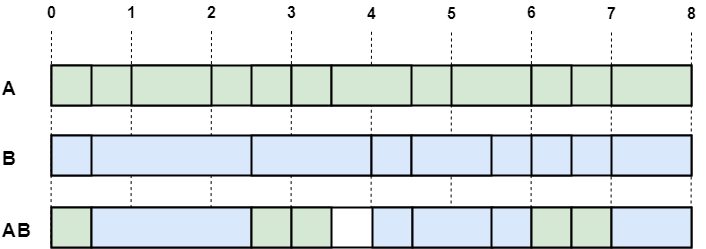
\includegraphics[width=0.9\linewidth]{init}
\end{center}

\begin{flushleft}
	\Large{\textbf{Rating}}
\end{flushleft}
\vspace{0.1cm}
\textbf{Based on the scale that the song tend to follow}
\begin{center}
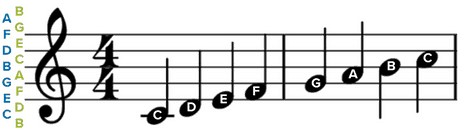
\includegraphics[width=0.6\linewidth]{scale}
\end{center}
\textbf{Zipf's law distance scores for Pitches and Intervals}
\begin{center}
	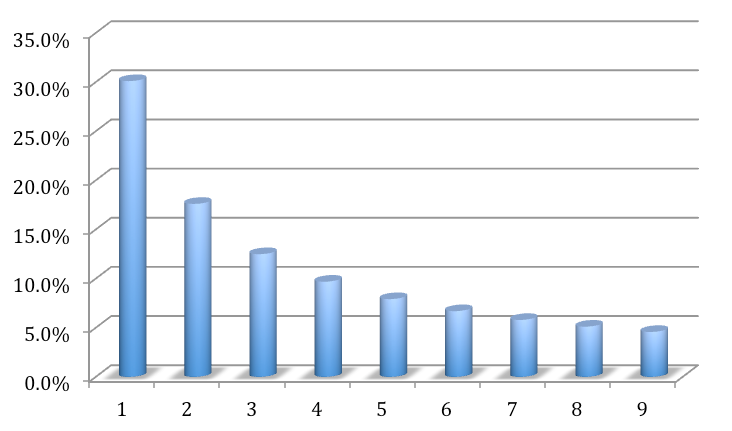
\includegraphics[width=0.6\linewidth]{zipfs}
\end{center}
\textbf{Neighbour pitch score:} counting the wrong intervals
\begin{center}
	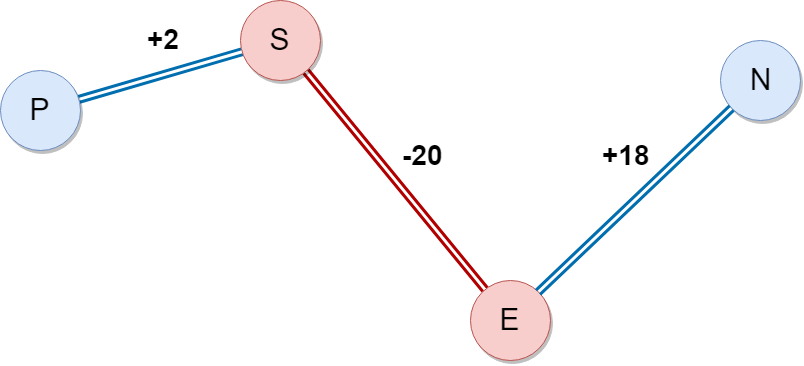
\includegraphics[width=0.6\linewidth]{Case1}
	\captionof{figure}{In this case, the note with label E is going to be transposed upwards.}
\end{center}
\textbf{Melody based scores:}
	\[ MelodyDirection(x) = \frac{\textit{Number of upwards intervals}}{\textit{Total number of intervals} } \]
	\[ DirectionStability(x) = \frac{\textit{Number of direction changes}}{\textit{Total number of intervals} } \]
	\[ UniquePitches(x) = \frac{\textit{Number of uniques pitches}}{\textit{Total number of pitches} } \]
\textbf{Measure relations \& repetition scores}

\begin{center}
	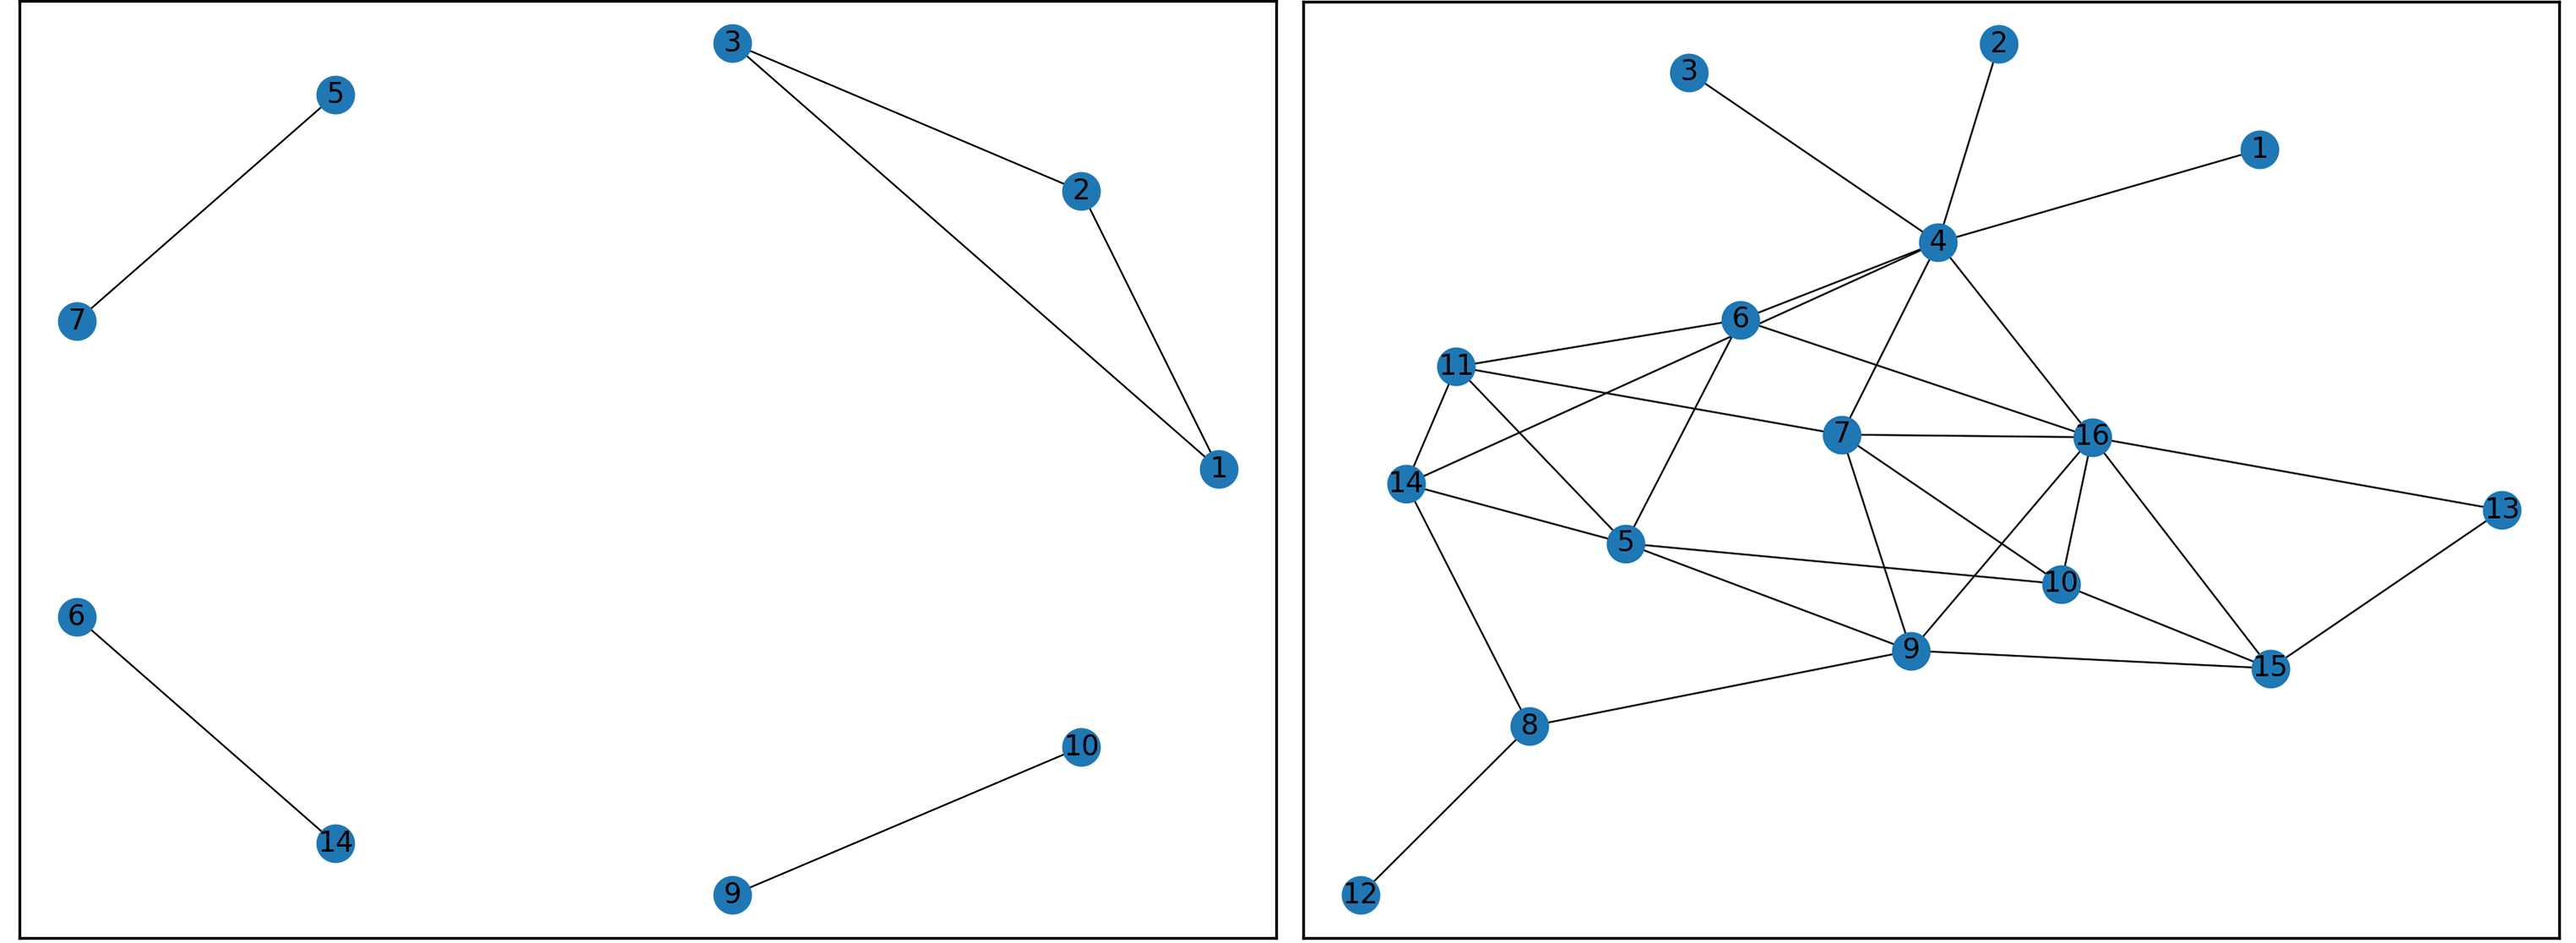
\includegraphics[width=\linewidth]{GodFather_1-2}
	\captionof{figure}{The measures of the  Godfather theme song represented on a graph with every node being a measure and every edge being the relation between them. The first represents graph the measures with the strong relations, the second with normal}
\end{center}
\Large{\textbf{Master-based measure structure sub-raters:} types, offsets, durations, pitches and intervals.}
\begin{center}
	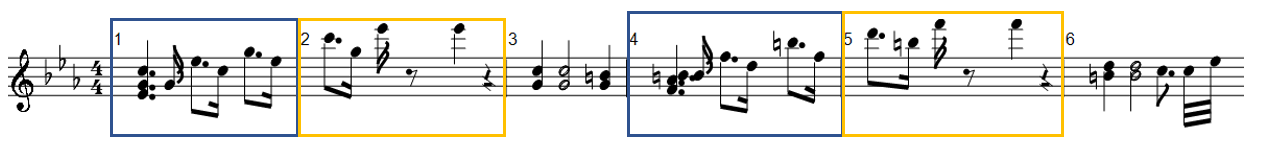
\includegraphics[width=\linewidth]{beethoven_measures}
	\captionof{figure}{The first 6 measures of Beethoven Op.10 No.1}
\end{center}
\Large{\textbf{Master-based absolute sub-raters}}
\begin{center}
	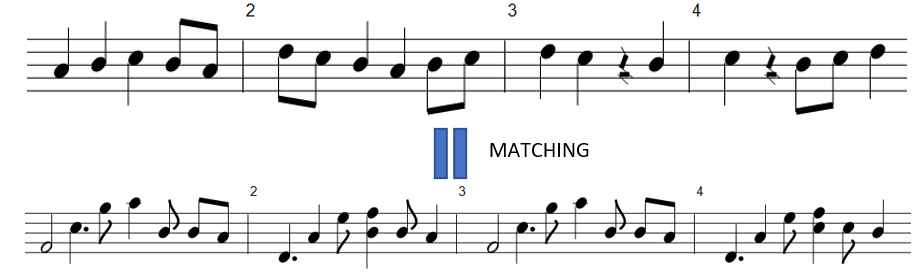
\includegraphics[width=1\linewidth]{absolute_matching}
\end{center}
\textbf{Total Rating:}
\LARGE\textbf{\[ R(x) = \sum_{S=1}^{n} S_{score} * S_{weight} \   \text{  (with S as sub-rater)}\]}
\begin{flushleft}
	\LARGE{\textbf{Mutations}}\\
\end{flushleft}
\Large{
\textbf{Measure mutations:} planned and random
\begin{enumerate} 
	\item \textbf{replacing} measures with others,
	\item \textbf{mixing} elements of two measures and
	\item \textbf{swapping} the location of two measures
\end{enumerate}
	\begin{flushleft}
		\Large{\textbf{Element mutations:}}
	\end{flushleft}
}
\begin{center}
	\includegraphics[width=0.7\linewidth]{mutations}
\end{center}

%----------------------------------------------------------------------------------------
%	RESULTS 
%----------------------------------------------------------------------------------------
\begin{flushleft}
	\LARGE{\textbf{Results}}
\end{flushleft}
\Large{First, the total rating of the fittest song will \textbf{decrease exponentially}. After a while it \textbf{stagnates around a fixed point} waiting for a \textbf{mutation} to have positive effect on its value.}
\begin{center}
	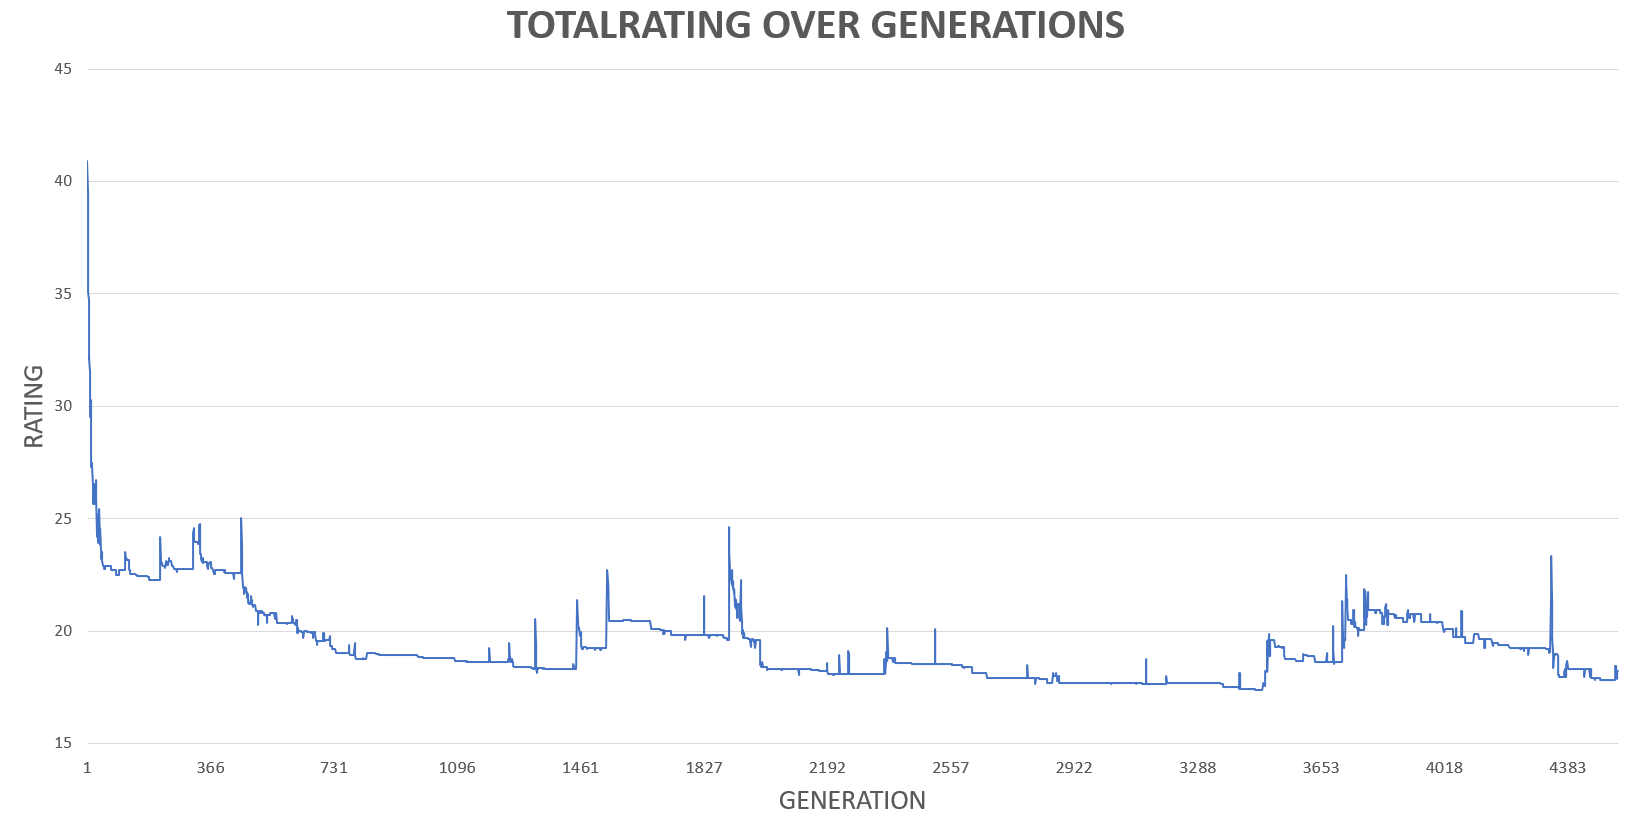
\includegraphics[width=1.05\linewidth]{total_rating_graph2}
	\captionof{figure}{Totalrating of the fittest song per generation plotted over 4531 generations}
\end{center}

\begin{flushleft}
	\LARGE{\textbf{Conclusions}}
\end{flushleft}
\begin{itemize}
	\item \Large \textbf{Strategic planning }can help improving the execution \textbf{speed}.
	\item Correct configuration of the \textbf{weights} is key for successful results.
	\item \textbf{More dimensions and layers} can be involved in the rating and mutation process. The\textbf{ more data }we can extract, the \textbf{closer} the results can be to the master. 
	\item Composing music with a genetic algorithm can be \textbf{effective} with the \textbf{necessary tools}.
\end{itemize}

\color{DarkSlateGray} % Set the color back to DarkSlateGray for the rest of the content

%----------------------------------------------------------------------------------------
%	FORTHCOMING RESEARCH
%----------------------------------------------------------------------------------------

%----------------------------------------------------------------------------------------
%	REFERENCES
%----------------------------------------------------------------------------------------


%----------------------------------------------------------------------------------------
%	ACKNOWLEDGEMENTS
%----------------------------------------------------------------------------------------


%----------------------------------------------------------------------------------------

\end{multicols}
\end{document}